% preamble with all definitions
\documentclass[12pt,letterpaper]{article}
\usepackage[utf8]{inputenc}
\usepackage[english]{babel}
\usepackage{amsmath}
\usepackage{amsfonts}
\usepackage{amssymb}
\usepackage{graphicx}
\usepackage{multirow}
\usepackage{fancyvrb}
\usepackage[breaklinks=true]{hyperref}
\usepackage[hyphenbreaks]{breakurl}
\hypersetup{
       pdfauthor = {Kim Siang Khaw},
        colorlinks=true, citecolor=blue, linkcolor=blue, bookmarksnumbered = true,
}
\usepackage[left=2cm,right=2cm,top=2cm,bottom=2cm]{geometry}

%%%%%%%Some style changes
\usepackage{caption}
\setlength{\captionmargin}{10mm}
\renewcommand\captionfont{\it}
\renewcommand\captionlabelfont{\bf}


\author{Wes Gohn, Tim Gorringe, Kim Siang Khaw}
\title{DAQ data structure for the Muon g-2 experiment}
\begin{document}

\maketitle

\abstract{This document outlines the DAQ data structure of the Muon g-2 experiment.}

\section{DAQ output in a nutshell}
The main DAQ framework for the Muon g-2 experiment is based on MIDAS [cite]. 

\section{MIDAS Bank list}

\begin{table}[htbp]
\centering
\caption{MIDAS bank list for the calorimetry data.}
\begin{tabular}{|c|c|c|c|}
\hline 
\multicolumn{3}{|c|}{Bank name}  & \multirow{2}{*}{Description} \\ \cline{1-3}
muon fill& laser fill & pedestal fill & \\
\hline
CA & LA & PA & AMC13 Header \\ 
\hline 
CB & LB & PB & WFD5 header \\ 
\hline 
CC & LC & PC & GPU timing data \\ 
\hline 
CF & LF & PF & GPU fitted data \\ 
\hline 
CH & LH & PH & Per crystal Q-method data (N-th event, end of run) \\ 
\hline 
CL & LL & PL & Clock data \\ 
\hline 
CP & LP & PP & Pedestal\\ 
\hline 
CQ & LQ & PQ & Per calo Q-method data (every event) \\ 
\hline 
CR & LR & PR & WFD5 raw data \\ 
\hline 
CT & LT & PT & T-method islands \\ 
\hline 
CZ & LZ & PZ & AMC13 CDF trailers \\ 
\hline 
\end{tabular} 
\end{table}


\begin{table}[htbp]
\centering
\caption{MIDAS bank list for auxiliary T/Q data. This is mainly for the fiber harps, quads and kickers.}
\begin{tabular}{|c|c|}
\hline 
Bank name  & Description \\
\hline
KH &  Per aux. detector channel Q-method data (N-th event, end of run)\\
\hline
KQ &  Per aux. detector Q-method data (every event)\\
\hline
KT & T-method data \\
\hline
\end{tabular} 
\end{table}

\begin{table}[htbp]
\centering
\caption{MIDAS bank list for the CCC data.}
\begin{tabular}{|c|c|}
\hline 
TTCA & AMC13 Header \\
\hline
TTCR & CCC AMC13 Payload\\
\hline
TTCZ & AMC13 Trailer \\
\hline
\end{tabular} 
\end{table}


\section{Bank contents}

This section details contents of each MIDAS bank. 

\begin{figure}[htbp]
\centering
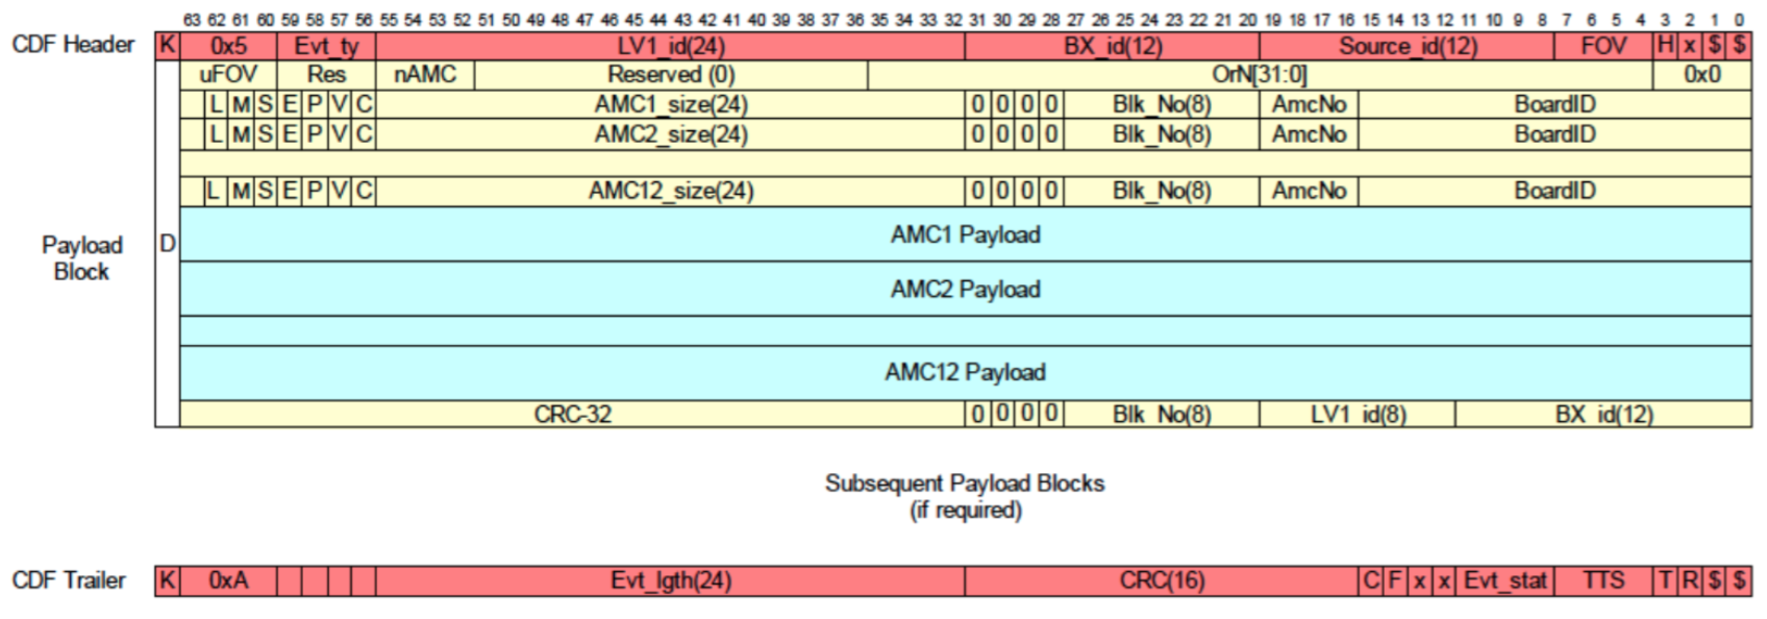
\includegraphics[width=\textwidth]{pics/AMC13ToDAQ.pdf} 
\caption{Data structure for AMC13 to DAQ.}\label{fig:AMC13ToDAQ}
\end{figure}

\begin{figure}[htbp]
\centering
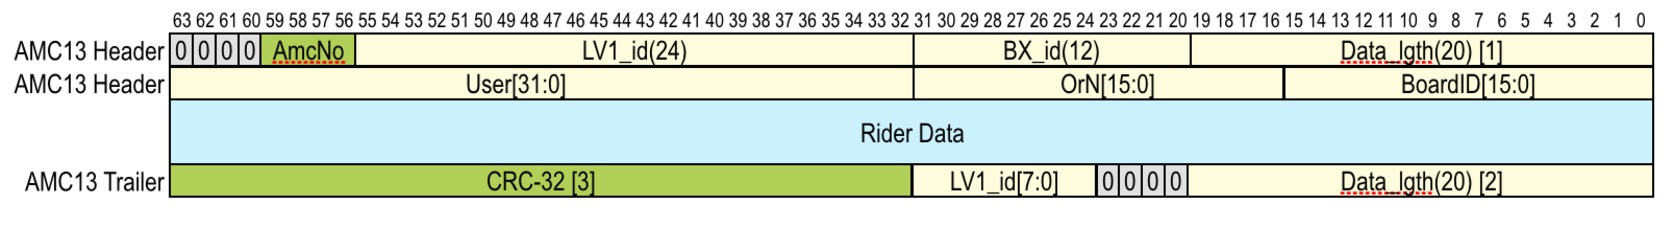
\includegraphics[width=\textwidth]{pics/RiderToAMC13.pdf} 
\caption{Data structure for Rider to AMC13.}\label{fig:RiderToAMC13}
\end{figure}

\begin{figure}[htbp]
\centering
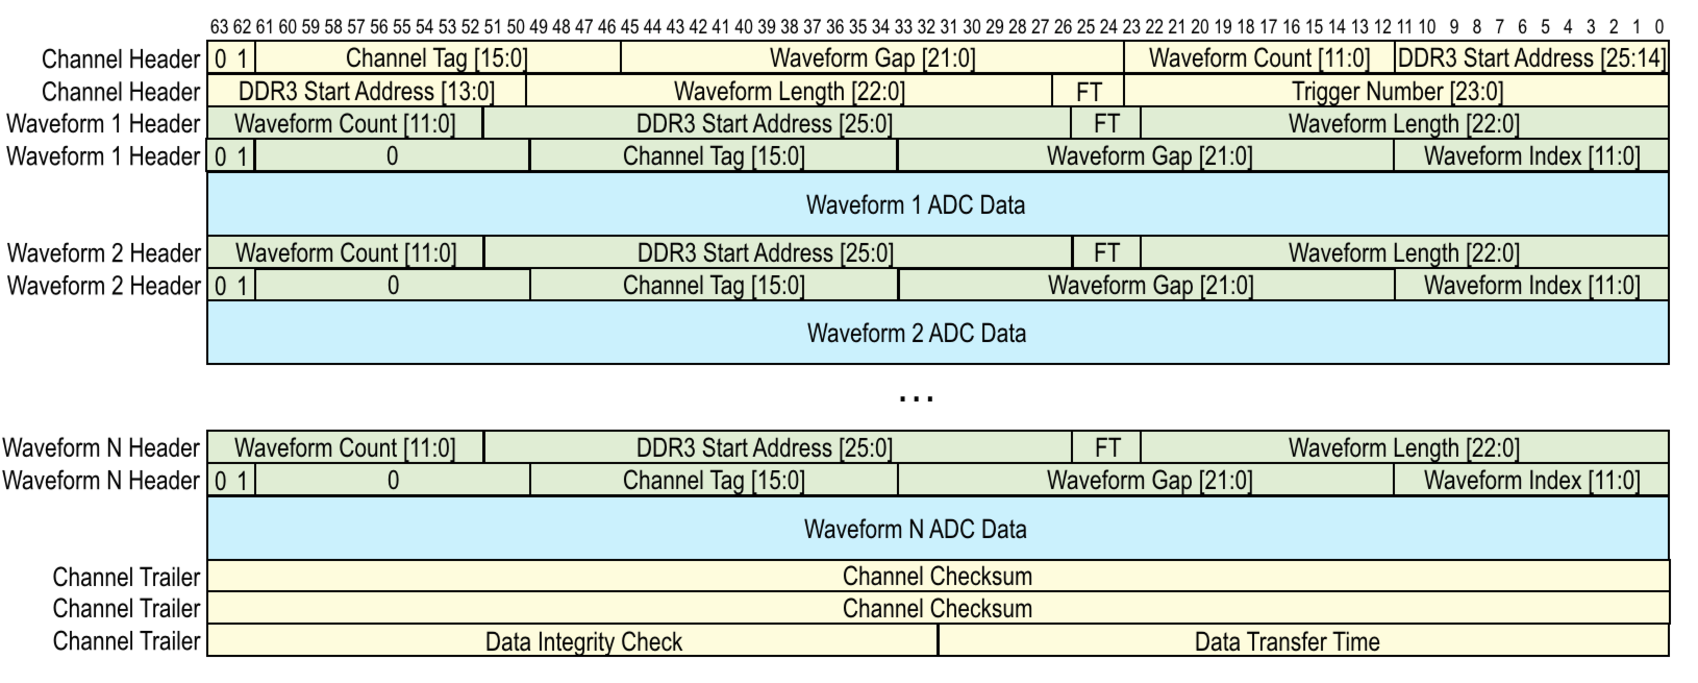
\includegraphics[width=\textwidth]{pics/RiderData.pdf} 
\caption{Data structure for Rider.}\label{fig:RiderData}
\end{figure}

\begin{figure}[htbp]
\centering
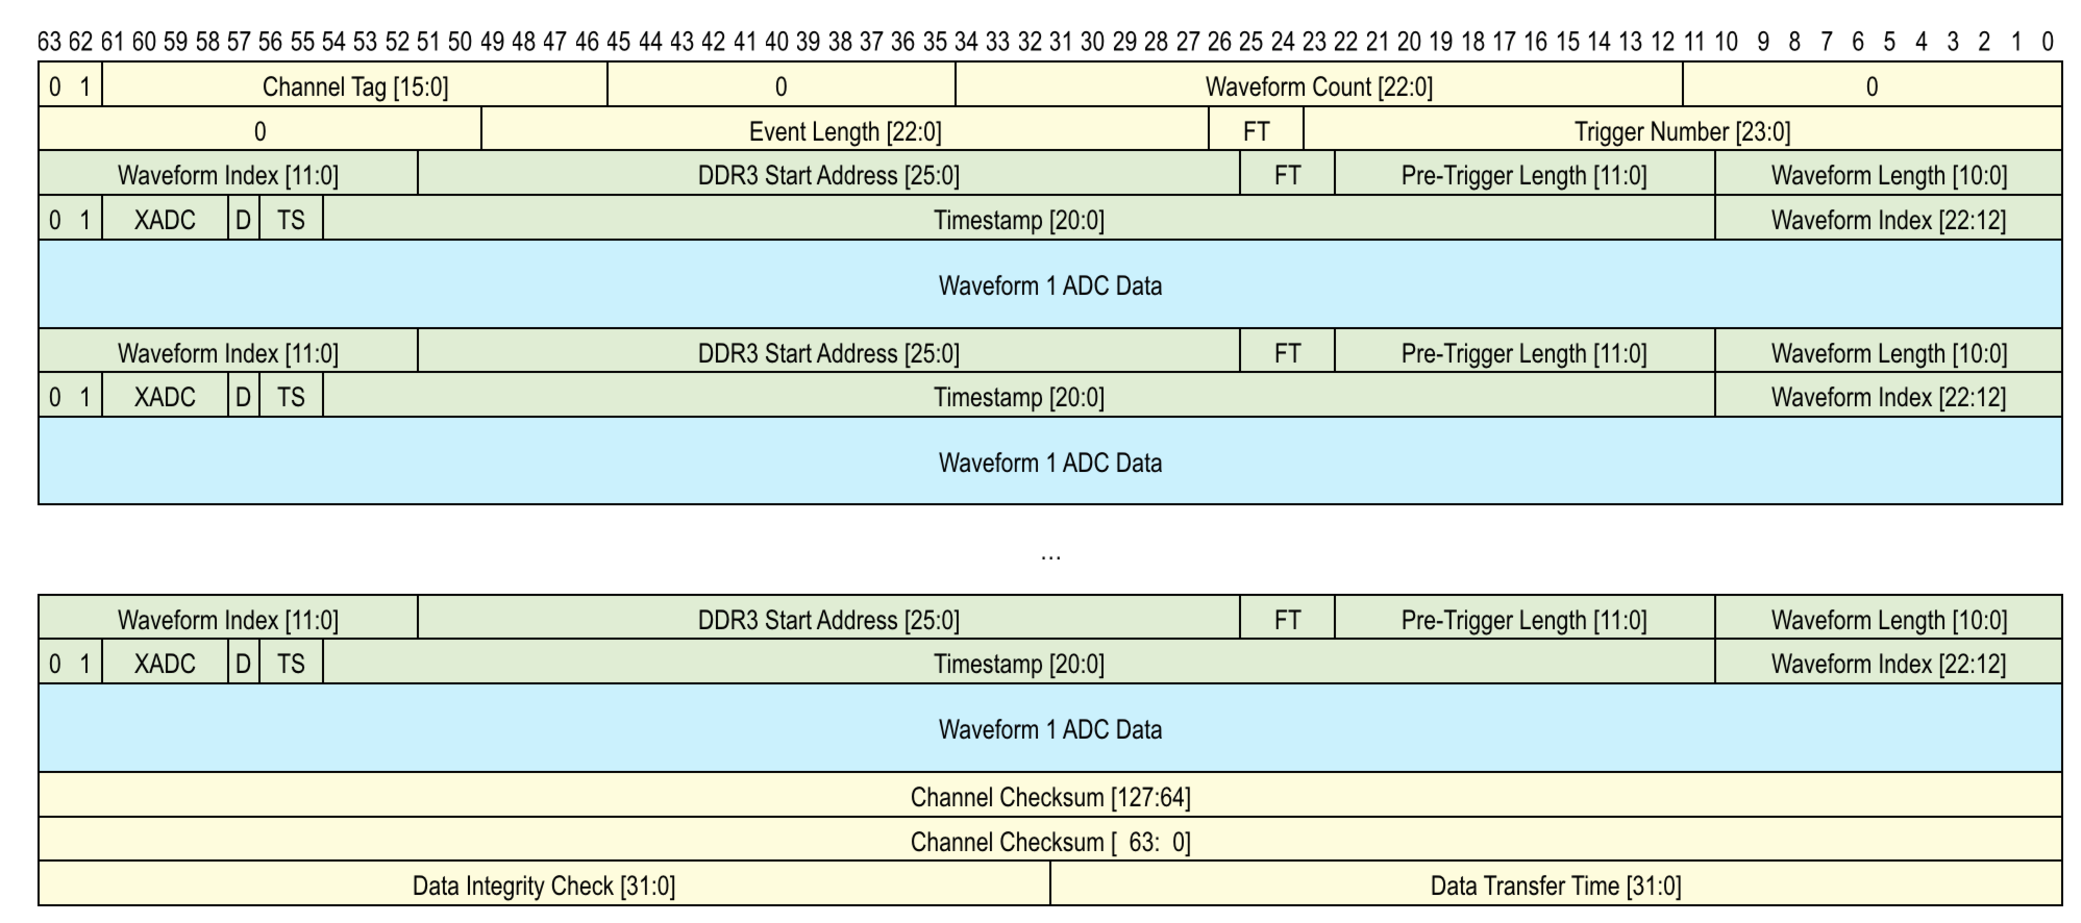
\includegraphics[width=\textwidth]{pics/AsyncRiderData.pdf} 
\caption{Data structure for asynchronous mode for Rider.}\label{fig:AsyncRiderData}
\end{figure}

\begin{figure}[htbp]
\centering
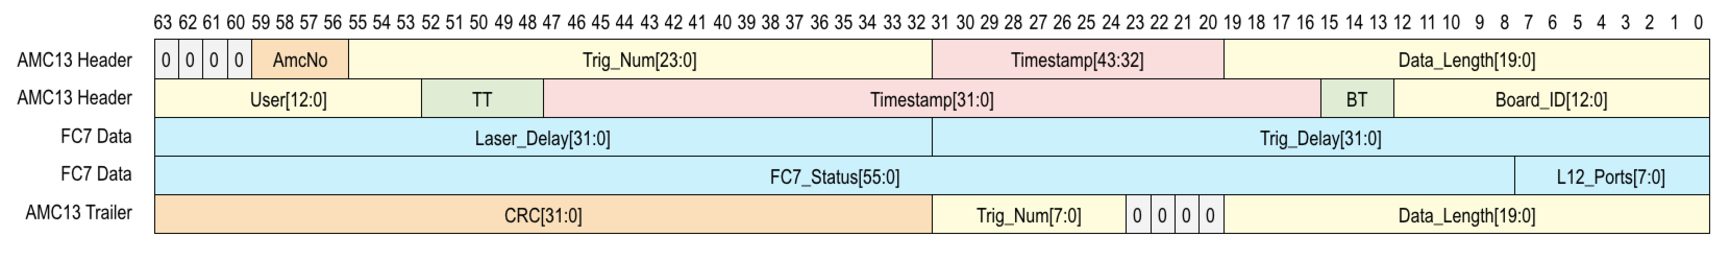
\includegraphics[width=\textwidth]{pics/EncoderFC7.pdf} 
\caption{Data structure for encoder FC7.}\label{fig:EncoderFC7}
\end{figure}


\begin{figure}[htbp]
\centering
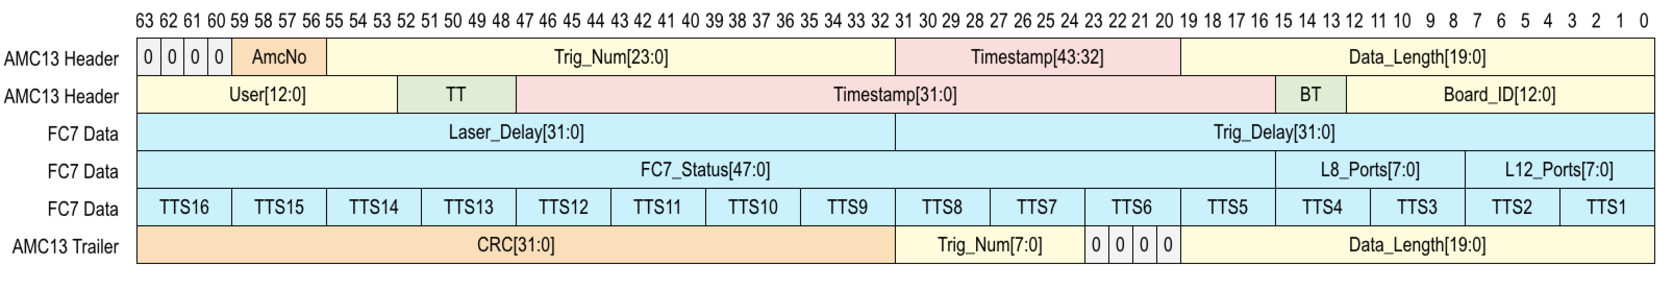
\includegraphics[width=\textwidth]{pics/FanoutFC7.pdf} 
\caption{Data structure for fanout FC7.}\label{fig:FanoutFC7}
\end{figure}


\section{C++ Parser}
Muon g-2 offline analysis framework relies on parsers in the gm2parser namespace hosted under repository gm2unpacker to decode the data.

\end{document}
